Während sich agile Praktiken im Hinblick auf die Softwareentwicklung auf eine kontinuierliche Planung, Flexibilität und eine schnelle Reaktion auf sich ändernde Kundenanforderungen fokussieren, können DevOps-Praktiken dazu verwendet werden, den Arbeitsfluss vom Kunden über die Entwicklung, den Betrieb und zurück kontinuierlich auszubauen und damit die Qualität und Belastbarkeit der Software zu steigern. \cite{fitzgerald_continuous_2014} \cite[S. 264]{tokarski_strategische_2018}

Die \textit{'Continuous Everything'}-Methoden spiegeln die Idee einer kontinuierlichen Verbesserung und Automatisierung innerhalb eines Devops-Prozesses wieder. 

Wie in der Abbildung zu erkennen ist, können sich diese Methoden auf merhrere Entwicklungszyklenphasen konzentrieren und werden in diesem Abschnitt im Einzelnen beschrieben.  

\begin{figure}[h]
    \centering
    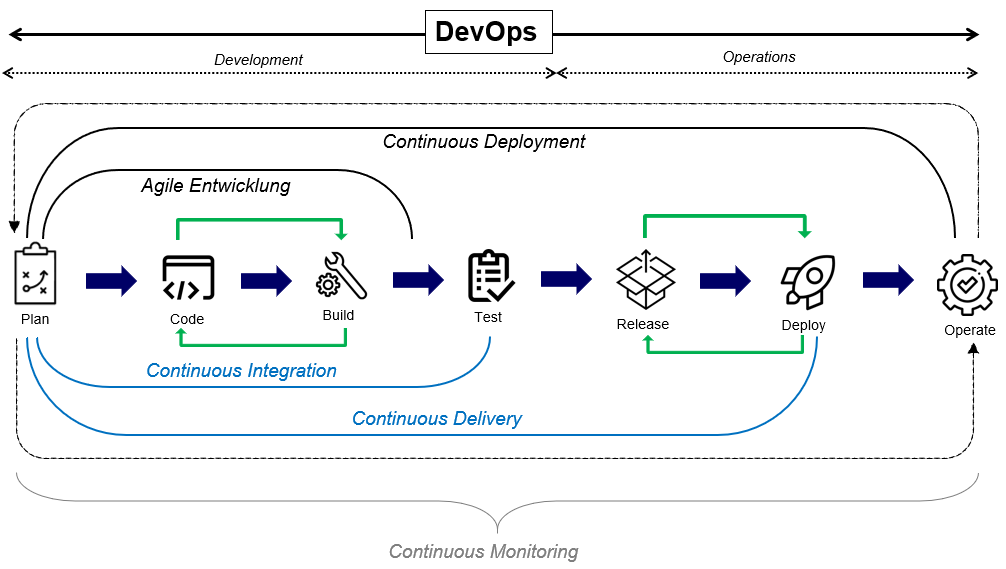
\includegraphics[scale=0.6]{Bilder/Continuous Everything.png}
    \caption{Continuous-Methoden innerhalb des Devops-Lebenszykluses, angelehnt an \cite[S. 16]{halstenberg_devops_2020}}
\end{figure}

\paragraph{Agile Entwicklung}

Die agile Entwicklung beschreibt die Verwendung von agilen Methoden innerhalb des Softwareentwicklungsprozesses als eine wesentliche Grundvoraussetzung für den DevOps-Prozess. 

Oftmals wird dieser Prozess auch als Continuous Planning (dt kontinuierliches Plannen) bezeichnet und reicht von der Phase des Planes bis zur Phase des Builds. \cite{fitzgerald_continuous_2014} 

Wie bereits in der Phase des Planens beschrieben, können agile Methoden wie Scrum und Kanban zum Einsatz kommen um die entsprechenden Ressourcen und die Entwicklungen während des ganzen Zeitraums zu planen und einzuteilen.

Inerhalb dieser Methode werden Features in kleinen Inkrementen geplant und entwickelt, um diese innerhalb eines Sprints umzusetzen und folglich die Durchlaufzeit bis zur Auslieferung kurzzuhalten. \cite[S. 266]{tokarski_strategische_2018} 

Infolgedessen beinhalten die Ergebnisse dieser Methode ausliefbare und getestete Funktionalitäten nach jedem Sprint. 

Continuous Planning gilt als ein ganzheitliches Unterfangen, dass ein engere Intergration zwischen Planung und Ausführung erfordert und an dem sowohl Kunden als auch die Entwickler beteiligt sind. \cite{fitzgerald_continuous_2014} 

Ziel ist es sicherzustellen, dass die Investitionsentscheidungen während des gesamten Lbenszykluses auf die Bedürfnisse des Kunden abgestimmt worden sind. 

\paragraph{Continuous Integration}

Die Methode des Continous Integration (dt. kontinuierliche Integration, kurz: CI) beschreibt grundsätzlich die Gewährleistung einer sicheren und lückenlosen Integration von Codeänderungen in die vorhandenen Umgebungen. \cite[S. 266]{tokarski_strategische_2018}  

Ziel ist es, die Qualität der Software sicherzustellen und schnelles Feedback über die Integrierbarkeit vor der Auslieferung zum Kunden zu erhalten. \cite[S. 266]{tokarski_strategische_2018} 

Kernelement stellt ein Versionsverwaltungssystem (auch: Repository) dar, dessen wesentliche Aufgabe es ist, den DevOps-Teams dabei zu helfen, den Code zu organisieren, Änderungen zu verfolgen und automasierte Tests zu ermöglichen. 

Zunächst werden neuer oder geänderter Code nach der Entwicklung und Prüfung regelmäßig und in möglichst kurzen Abständen in einem gemeinsamen Repository gemergt (dt. zusammengeführt). \cite[S. 13-16]{sharma_devops_2017}

In diesem Zuge wird der Code automatisiert in einem Build kompiliert. 

Die neu erstellten Artefakte, als Ergebnis des Builds, werden in eine lauffähige Umgebung integriert und automasiert getestet. 

Damit soll sichergestellt werden, ob die neue Codeänderung einer Komponente im Kontext der gesamten Anwendung lauffähig ist. 

Dies ist essentiell für den Prozess, da häufig viele Entwickler an der Codebasis mit leicht unterschiedlichen Versionen arbeiten und daher überprüft werden kann, ob die verschiedenen Änderungen richtig zusammenarbeiten. \cite[S. 69]{verona_practical_2016} 

Aufgrund des regelmäßigen Integrieren der Codeänderungen wird gewährleistet, dass häufige automatisierte Tests durchführt werden, den Entwicklern stets der aktuellste Code zur Verfügung steht und Entwickler nicht darauf warten müssen, einzelne Codeabschnitte am Tag der Veröffentlichung auf einmal zu integrieren. \cite{thedev_eight_2019} 

Durch die entstehende Flexibilität und Geschwindigkeit können Fehler schneller und leichter behoben werden, da die Programmbestandteile kleiner und weniger komplex sind und das Debugging insgesamt sinkt. \cite{thedev_eight_2019}

Darüber hinaus werden Änderungen sichtbarer und bilden eine starke Grundlage für zukünftige Änderungen. 

Insgesamt umfasst CI Schritte wie die Codekompilierung, die Durchführung von Unit- und Akzeptanztests, die Validierung der Codeabdeckung, die Überprüfung der Einhaltung von Codierungsstandards und die Erstellung von Bereitstellungspaketen. \cite{fitzgerald_continuous_2014} 

\paragraph{Continuous Delivery}

Bei dem Ansatz des Continuous Delivery handelt es sich um die nächste Stufe des Continuous Integration. 

Dabei werden die fehlerfreien Builds automatisch in produktionsähnlichen Testumgebungen bereitgestellt, in denen funktionale Tests, Integrationstests, Leistungstests und Sicherheitstests durchgeführt werden können, um zu bewerten, wie sich diese verhalten.

Zunächst werden die entstehenden Builds auf ihre Funktionalität, Stabilität und andere nicht-funktionale Anforderungen getestet, indem diese in einen produktionsähnlichen Staging- oder Testbereich bereitgestellt werden.

Die Vorgehensweise der regelmäßigen Übergabe der entwickelten Funktionalität in den Testbereich und in den Betrieb zur Validierung und potenziellen Freigabe an den Kunden wird letztlich als Continuous Delivery

Der Ansatz des Continuous Delivery erfordert die Erstellung einer Delivery-Pipeline. 

Da die Continuous Integration regelmäßig Builds erzeugt, müssen diese zeitnah in andere Umgebungen in der Delivery-Pipeline weitergeleitet werden.

Builds müssen in der Testumgebung bereitgestellt werden, um Tests durchzuführen, in der Integrationsumgebung für Integrations-Builds und Integrationstests, und so weiter, bis hin zur Produktion.

Continuous Delivery erleichtert die Bereitstellung von Anwendungen von einer Umgebung zur nächsten, je nach Bedarf.

Continuous Delivery erfordert die Orchestrierung der Bereitstellung von Code, Inhalten, Anwendungen, Middleware- und Umgebungskonfigurationen sowie Prozessänderungen. 


Nach der Verschiebung in eine Staging-Umgebung muss entschieden werden, ob das Build in die Produktion verlagert werden kann oder nochmal bewertet werden muss. 

Durch die Codefreigabe in kleinen Artefakten können Engpässe vermieden und ein kontinuierlicher Fluss sichergestellt werden. 


%Wolff
Grundlage für CD ist der Aufbau einer Continuous-Delivery-Pipeline, die das Ausrollen der Software weitgehend automatisiert und so einen reproduzierbaren Prozess für die Bereitstellung neuer Releases darstellt. 


%Bloomberg
Dabei werden die fehlerfreien Builds automatisch in produktionsähnlichen Testumgebungen bereitgestellt, in denen funktionale Tests, Integrationstests, Leistungstests und Sicherheitstests durchgeführt werden können.

Die CD-Pipeline wird durch jedes neue Build-Artefakt ausgelöst, das im Repository veröffentlicht wird. Im Idealfall stellt die CD-Pipeline die Arbeit auch automatisch in die Produktionsumgebung bereit, wenn alle Tests bestanden sind. 

Falls ein Test in der Pipeline fehlschlägt, wird das Deployment gestoppt und das Team wird darüber informiert, dass mit diesem Build etwas nicht stimmt. 

Die Anwendung von Continuous Delivery verändert den Release-Management-Prozess rund um die Anwendung radikal. 

Die CD-Pipeline reduziert die Komplexität der Release-Prozesse, indem sie die Lieferrisiken verringert und die Geschwindigkeit der Lieferung und des Feedbacks erhöht. 

Die Änderungen, die an die Produktion geliefert werden, sind so klein wie möglich, gründlich getestet und werden so oft und so automatisch wie möglich bereitgestellt.

Die technische Umsetzung von automatisiertem CD ist jedoch nicht einfach. So kann es beispielsweise einige Zeit dauern, bis der Grad der Testautomatisierung erreicht ist, der es dem Team ermöglicht, sich darauf zu verlassen, dass die Bereitstellung sicher ist. Daher ist in einigen Fällen ein menschliches Eingreifen in der letzten Phase erforderlich, in der die Änderung in die Produktion übernommen wird. (Verona 2016, 16-17.) 










Continuous Delivery ist eine Erweiterung von Continuous Integration, die den Prozess der BEreitstellung eiens neues Builds in der Produktion automatisiert.

Ziele sind: 
1. Automatisierte Tests für jeden neuen Build durchzuführen, um zu überprüfen, ob die Builds für die Produktion bereit sind, und diejenigen, die es nicht sind, zu verwerfen.
2.Die automatische Bereitstellung und Konfiguration von Bereitstellungsumgebungen sowie das Testen dieser Umgebungen auf Stabilität, Leistung und Sicherheitskonformität zu verwalten. 
3. Bereitstellung einer neuen Version für die Produktion, wenn diese von der Organisation genehmigt und manuell ausgelöst wurde.


Continuous Delivery ist auf die Test- und Release-Phasen der Pipeline abgestimmt und ermöglicht es Unternehmen, die Freigabe neuer Builds in beliebigen Abständen manuell auszulösen.




Continuous Delivery (CD) ist der nächste logische Schritt von CI. Codeänderungen werden automatisch erstellt, getestet und für die Freigabe in die Produktion verpackt. Ziel ist es, Aktualisierungen schnell und nachhaltig an die Benutzer weiterzugeben.


Nach den CI-Schritten wird automatisiert sichergestellt, dass die neu entstandene Version dafür bereit ist, im Produktivbetrieb eingesetzt zu werden. Der CI-Prozess wird um den
Schritt Akzeptanztest / Staging / Performancetests erweitert. In diesem wird die neue Version
unter anderem in einer der Produktivumgebung so nahe wie möglich nachempfundenen
Testumgebung (Staging-Umgebung) auf Herz und Nieren getestet 


\paragraph{Continuous Deployment}

\paragraph{Continuous Monitoring}

\paragraph{Infrastructur-as-a-Code}













Unter Continuous Integration versteht man im Wesentlichen den Build-Prozess und die darauffolgenden automatisierten Tests, die durch das Einchecken von neuen Code Changes in das Software Repository ausgelöst werden. Dies sorgt dafür, dass schnell klar ist, ob neue Codeänderungen einer Komponente im Gesamtkontext der Anwendung lauffähig sind. Durch das häufige Testen ist außerdem die Zuordnung des Fehlers zur verursachenden Änderung leichter herzustellen.\\

Der Continuous Integration-Prozess ist nach den Änderungen am Source Code und der Ausführung der Tests abgeschlossen und beginnt daraufhin wieder von vorn. Continuous Delivery setzt an dieser Stelle an und erweitert den Feedback-Zyklus bis in die Produktion. Erst wenn die Anwendung in die Produktion deployt wurde und dem Kunden zur Verfügung steht, ist die "Definition of Done" erfüllt. Vor diesem Hintergrund wird Continuous Delivery auch als finale Stage oder "letzte Meile" von Continuous Integration bezeichnet.\\

Continuous Deployment (das andere „CD“) kann sich auf die automatische Freigabe von Entwickleränderungen vom Repository zur Produktivphase beziehen, wo sie direkt vom Kunden genutzt werden können. Dieser Vorgang soll der Überlastung von Operations-Teams bei manuellen Prozessen entgegenwirken, die die Anwendungsbereitstellung verlangsamen. Continuous Development baut die Vorteile der Continuous Delivery aus, indem auch noch die nächste Phase der Pipeline automatisiert wird.\\

Unter Deployment Pipeline versteht man einen Prozess, der die Schritte Build, Test und Deployment des Softwareauslieferungsprozesses über mehrere Stages hinweg automatisiert durchläuft.\\


Nachfolgend werden verschiedene Testarten und Begriffe erläutert: Staging-Umgebung, Unit Test, Acceptance Test, Integration Test, Smoke Test:




















Gemäß des DevOps-Konzepts werden die Grundsätze des DevOps-Ansatzes durch den Aufbau einer Bereitstellungspipeline (engl. Deployment Pipeline) durchgesetzt. 

Die Deployment-Pipeline besteht im Wesentlichen aus mehreren Continuous Integration und Continuous Delivery-Pipelines und kann als eine automatisierte Implementierung der Build-, Test-, Deploymment- und Release-Prozesse einer Anwendung definiert werden. 

Mit der Deployment-Pipeline werden drei Ziele verfolgt. \cite[S. 3 - 4]{humble_continuous_2011} 

Zunächst ist jeder Schritt des Prozesses angefangen bei der Erstellung, des Einsatzes, des Testens und der Softwarefreigabe (End-to-End-Prozess) für alle sichtbar, wodurch die gesamte Zusammenarbeit gefördert wird. 

Weiterhin wird das Feedback verbessert, indem die Probleme sehr zeitnah im Prozess erkannt und behoben werden können. 

Darüber hinaus ist es jedem DevOps-Team möglich, alle Softwareversionen in jeder beliebigen Umgebung durch einen vollständig automatisierten Prozess bereitzustellen und freizugeben.






Wie bereits beschrieben ist ein wesentlicher Baustein des DevOps-Konzepts die Automatisierung. 

Oftmals bergen manuelle Arbeiten die Gefahr einer hohen Fehleranfälligkeit, zeitliche Unberechenbarkeit und schwerer Reproduzierung, wodurch insbesondere im Softwarebereitsstellungsprozess wenig Zeit für priorisierte Aufgaben bleiben. 

Um die Rolle der Automatisierung voranzutreiben und zu etablieren, sollten möglichst viele vollautomatisierte Deployments auf die Produktivumgebung aufgesetzt werden.   

In diesem Rahmen müssen DevOps-Teams Deployments. bzw Build-Pipelines aufbauen, um alle Änderungen am System, am Code oder an der Infrastruktur, mittels Pipeline zu automatisieren. 










Eine Deployment-Pipeline ist im Wesentlichen eine automatisierte Implementierung des Build-, Deployment-, Test- und Release-Prozesses Ihrer Anwendung. Jedes Unternehmen wird sich in der Implementierung seiner Deployment-Pipelines unterscheiden, je nach dem Wertstrom für die Freigabe von Software, aber die Prinzipien, die ihnen zugrunde liegen, unterscheiden sich nicht. Ein Beispiel für eine Bereitstellungspipeline ist in Abbildung 1.1 dargestellt.



Die Funktionsweise der Deployment-Pipeline lässt sich wie folgt zusammenfassen. Jede Änderung, die an der Konfiguration, dem Quellcode, der Umgebung oder den Daten einer Anwendung vorgenommen wird, löst die Erstellung einer neuen Instanz der Pipeline aus. 

Einer der ersten Schritte in der Pipeline ist die Erstellung von Binärdateien und Installationsprogrammen. Der Rest der Pipeline führt eine Reihe von Tests mit den Binärdateien durch, um zu beweisen, dass sie freigegeben werden können. 

Jeder Test, den der Freigabekandidat besteht, gibt uns mehr Sicherheit, dass diese bestimmte Kombination aus Binärcode, Konfigurationsinformationen, Umgebung und Daten funktionieren wird. 

Wenn der Freigabekandidat alle Tests besteht, kann er freigegeben werden. Die Deployment-Pipeline hat ihre Grundlage im Prozess der kontinuierlichen Integration und ist im Wesentlichen das Prinzip der kontinuierlichen Integration, das zu seinem logischen Abschluss gebracht wurde. 



